\documentclass[a4paper,12pt]{article} % добавить leqno в [] для нумерации слева
\usepackage[a4paper,top=1.3cm,bottom=2cm,left=1.5cm,right=1.5cm,marginparwidth=0.75cm]{geometry}
%%% Работа с русским языком
\usepackage{cmap}					% поиск в PDF
\usepackage{mathtext} 				% русские буквы в фомулах
\usepackage[T2A]{fontenc}			% кодировка
\usepackage[utf8]{inputenc}			% кодировка исходного текста
\usepackage[english,russian]{babel}	% локализация и переносы

\usepackage{graphicx}

\usepackage{wrapfig}
\usepackage{tabularx}

\usepackage{hyperref}
\usepackage[rgb]{xcolor}
\hypersetup{
colorlinks=true,urlcolor=blue
}
\usepackage{multirow}
\usepackage{hhline}


%%% Дополнительная работа с математикой
\usepackage{amsmath,amsfonts,amssymb,amsthm,mathtools} % AMS
\usepackage{icomma} % "Умная" запятая: $0,2$ --- число, $0, 2$ --- перечисление

%% Номера формул
\mathtoolsset{showonlyrefs=true} % Показывать номера только у тех формул, на которые есть \eqref{} в тексте.

%% Шрифты
\usepackage{euscript}	 % Шрифт Евклид
\usepackage{mathrsfs} % Красивый матшрифт

%% Свои команды
\DeclareMathOperator{\sgn}{\mathop{sgn}}

%% Перенос знаков в формулах (по Львовскому)
\newcommand*{\hm}[1]{#1\nobreak\discretionary{}
{\hbox{$\mathsurround=0pt #1$}}{}}

\begin{document}
	
	\begin{titlepage}
	\begin{center}
		{\large МОСКОВСКИЙ ФИЗИКО-ТЕХНИЧЕСКИЙ ИНСТИТУТ (НАЦИОНАЛЬНЫЙ ИССЛЕДОВАТЕЛЬСКИЙ УНИВЕРСИТЕТ)}
	\end{center}
	\begin{center}
		{\large Физтех-школа электроники, фотоники и молекулярной физики}
	\end{center}
	
	
	\vspace{4.5cm}
	{\huge
		\begin{center}
			{Лабораторная работа 4.3.2}\\
			Дифракция света на ультразвуковой волне в жидкости
		\end{center}
	}
	\vspace{2cm}
	\begin{flushright}
		{\LARGE Салтыкова Дарья \\
			\vspace{0.5cm}
			Б04-105}
	\end{flushright}
	\vspace{8cm}
	\begin{center}
		Долгопрудный 2023
	\end{center}
\end{titlepage}

\section{Введение}

\noindent \textbf{Цель работы:} изучение дифракции света на синусоидальной акустической решетке и наблюдение фазовой решетки методом темного поля.

\medskip
	
\noindent \textbf{В работе используются:} оптическая скамья, осветитель, два длиннофокусных объектива, кювета с жидкостью, кварцевый излучатель с микрометрическим винтом, генератор звуковой частоты, линза, вертикальная нить на рейтере, микроскоп.
	

\section{Теоретические сведения}

\noindent При прохождении ультразвуковой волны через жидкость в ней возникают периодические неоднородности коэффициента преломления, создается фазовая решетка, которую мы считаем неподвижной ввиду малости скорости звука относительно скорости света. Показатель преломления n изменяется по закону:
	
	\begin{equation}\label{}
	n = n_0 (1 + m \cos \Omega x)
	\end{equation}
	
\noindent Здесь $ \Omega = 2 \pi / \Lambda $ --- волновое число для ультразвуковой волны, $ m $ --- глубина модуляции $ n $ $ (m \ll 1 $).

\medskip
	
\noindent Положим фазу $ \phi $ колебаний световой волны на передней стенке кюветы равной нулю, тогда на задней поверхности она равна:
	
	\begin{equation}\label{}
	\phi  = k n L = \phi_0 (1 + m \cos \Omega x)
	\end{equation}
	
\noindent Здесь $ L $ --- толщина жидкости в кювете, $ k = 2 \pi / \lambda $ --- волновое число для света.

\medskip
	
\noindent После прохождения через кювету световое поле есть совокупность плоских волн, распространяющихся под углами $ \theta $, соответствующими максимумам в дифракции Фраунгофера:
	
\begin{minipage}{0.5\textwidth}
\begin{equation}\label{}	
	\Lambda \sin \theta_m = m \lambda
\end{equation}

\noindent Этот эффект проиллюстрирован на рисунке 1.

\medskip

\noindent Зная положение дифракционных максимумов, по формуле (1) легко определить длину ультразвуковой волны, учитывая малость $ \theta $: $ \sin \theta \approx \theta \approx l_m /F  $, где $ l_m $ --- расстояние от нулевого до последнего видимого максимума, $ F $ --- фокусное расстояние линзы. Тогда получим:
	
	\begin{equation}\label{}
	 \Lambda = m \lambda F/ l_m 
	\end{equation}
	
\noindent Скорость ультразвуковых волн в жидкости, где $ \nu $ --- частота колебаний излучателя:
	
\begin{equation}\label{}
	v = \Lambda \nu 
\end{equation}


\end{minipage}	
\begin{minipage}{0.47\textwidth}
		\begin{center}
		
		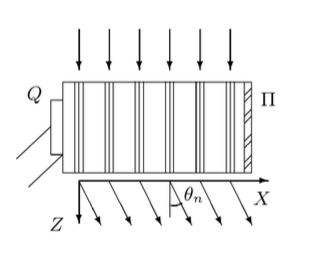
\includegraphics[width=0.9\textwidth]{1.png}
		
		Рис. 1. Дифракция световых волн на акустической решетке
		\label{diff}
		
		\end{center}

\end{minipage}	

\section{Экспериментальная установка}

\subsection{Определение скорости ультразвука по дифракционной картине}

\noindent Схема установки приведена на рисунке 2. Источник света Л через светофильтр Ф и конденсор К освещает вертикальную щель $ S $, находящуюся в фокусе объектива $ O_1 $. После объектива параллельный световой пучок проходит через кювету С перпендикулярно акустической решетке, и дифракционная картина собирается в фокальной плоскости объектива $ O_2 $ , наблюдается при помощи микроскопа М.

\medskip

\noindent Настройку установки будем произведить с зеленым фильтром, далее в работе будем использовать красный.

\begin{center}
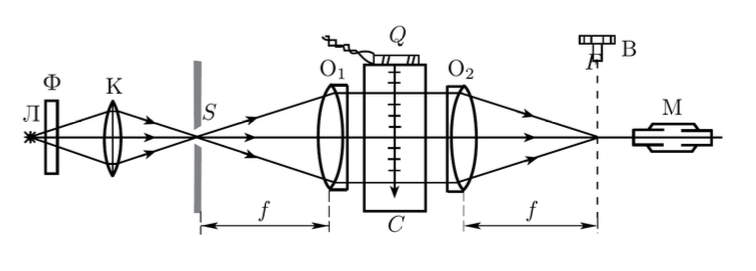
\includegraphics[width=0.7\textwidth]{2.png}

Рис. 2. Установка для наблюдения дифракции на акустической решетке
\label{shema1}
\end{center}

\noindent Параметры установки: фокусное расстояние объектива $  O_2  $ $ F = 30 $ см, одно деление винта микроскопа составляет 4 мкм, погрешность измерений примем равной  $ \sigma = $ 2 деления, или 8 мкм.

\subsection{Определение скорости ультразвука методом темного поля}

\noindent Для наблюдения акустической решетки используется метод темного поля, который заключается в устранении центрального дифракционного максимума с помощью непрозрачного экрана. Схема установки показана на рисунке.

	\begin{center}

	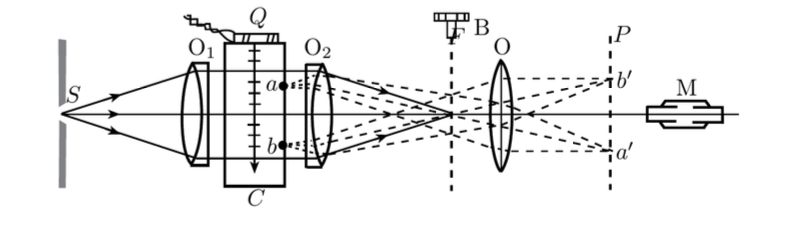
\includegraphics[width=0.7\textwidth]{3.png}
	
	Рис. 3. Установка для наблюдения дифракции методом темного поля
	\label{shema2}
\end{center}

\section{Ход работы}

\subsection{Определение скорости ультразвука по дифракционной картине}

\noindent 1. Проведя предварительную настройку, получим в поле зрения микроскопа систему дифракционных полос.

\medskip

\noindent 2. Определим положение нескольких дифракционных максимумов с помощью микрометрического винта отсчетного устройства. Повторим измерения для нескольких рабочих частот.

\begin{table}[!h]
\begin{tabular}{|lllllll|}
\hline
\multicolumn{7}{|c|}{$\nu   = 1,227 \text{ МГц}$}                                                                                                                                  \\ \hline
\multicolumn{1}{|l|}{m}                 & \multicolumn{1}{l|}{0} & \multicolumn{1}{l|}{1}   & \multicolumn{1}{l|}{2}   & \multicolumn{1}{l|}{3}   & \multicolumn{1}{l|}{4}   & 5   \\ \hline
\multicolumn{1}{|l|}{$x_m, \text{мкм}$} & \multicolumn{1}{l|}{0} & \multicolumn{1}{l|}{164} & \multicolumn{1}{l|}{344} & \multicolumn{1}{l|}{500} & \multicolumn{1}{l|}{676} & 844 \\ \hline
\end{tabular}
\end{table}

\begin{table}[!h]
\begin{tabular}{|llllll|}
\hline
\multicolumn{6}{|c|}{$\nu   = 2,881 \text{ МГц}$}                                                                                                         \\ \hline
\multicolumn{1}{|l|}{m}                 & \multicolumn{1}{l|}{0} & \multicolumn{1}{l|}{1}   & \multicolumn{1}{l|}{2}   & \multicolumn{1}{l|}{3}    & 4    \\ \hline
\multicolumn{1}{|l|}{$x_m, \text{мкм}$} & \multicolumn{1}{l|}{0} & \multicolumn{1}{l|}{340} & \multicolumn{1}{l|}{680} & \multicolumn{1}{l|}{1120} & 1528 \\ \hline
\end{tabular}
\end{table}

\newpage

\begin{table}[!h]
\begin{tabular}{|llll|}
\hline
\multicolumn{4}{|c|}{$\nu   = 4,60 \text{ МГц}$}                                                   \\ \hline
\multicolumn{1}{|l|}{m}                 & \multicolumn{1}{l|}{0} & \multicolumn{1}{l|}{1}   & 2    \\ \hline
\multicolumn{1}{|l|}{$x_m, \text{мкм}$} & \multicolumn{1}{l|}{0} & \multicolumn{1}{l|}{560} & 1440 \\ \hline
\end{tabular}
\end{table}

\noindent 3. По данным таблиц построим график зависимости координаты $x_m$ от порядка $m$.

\begin{figure}[!h]
 	\centering	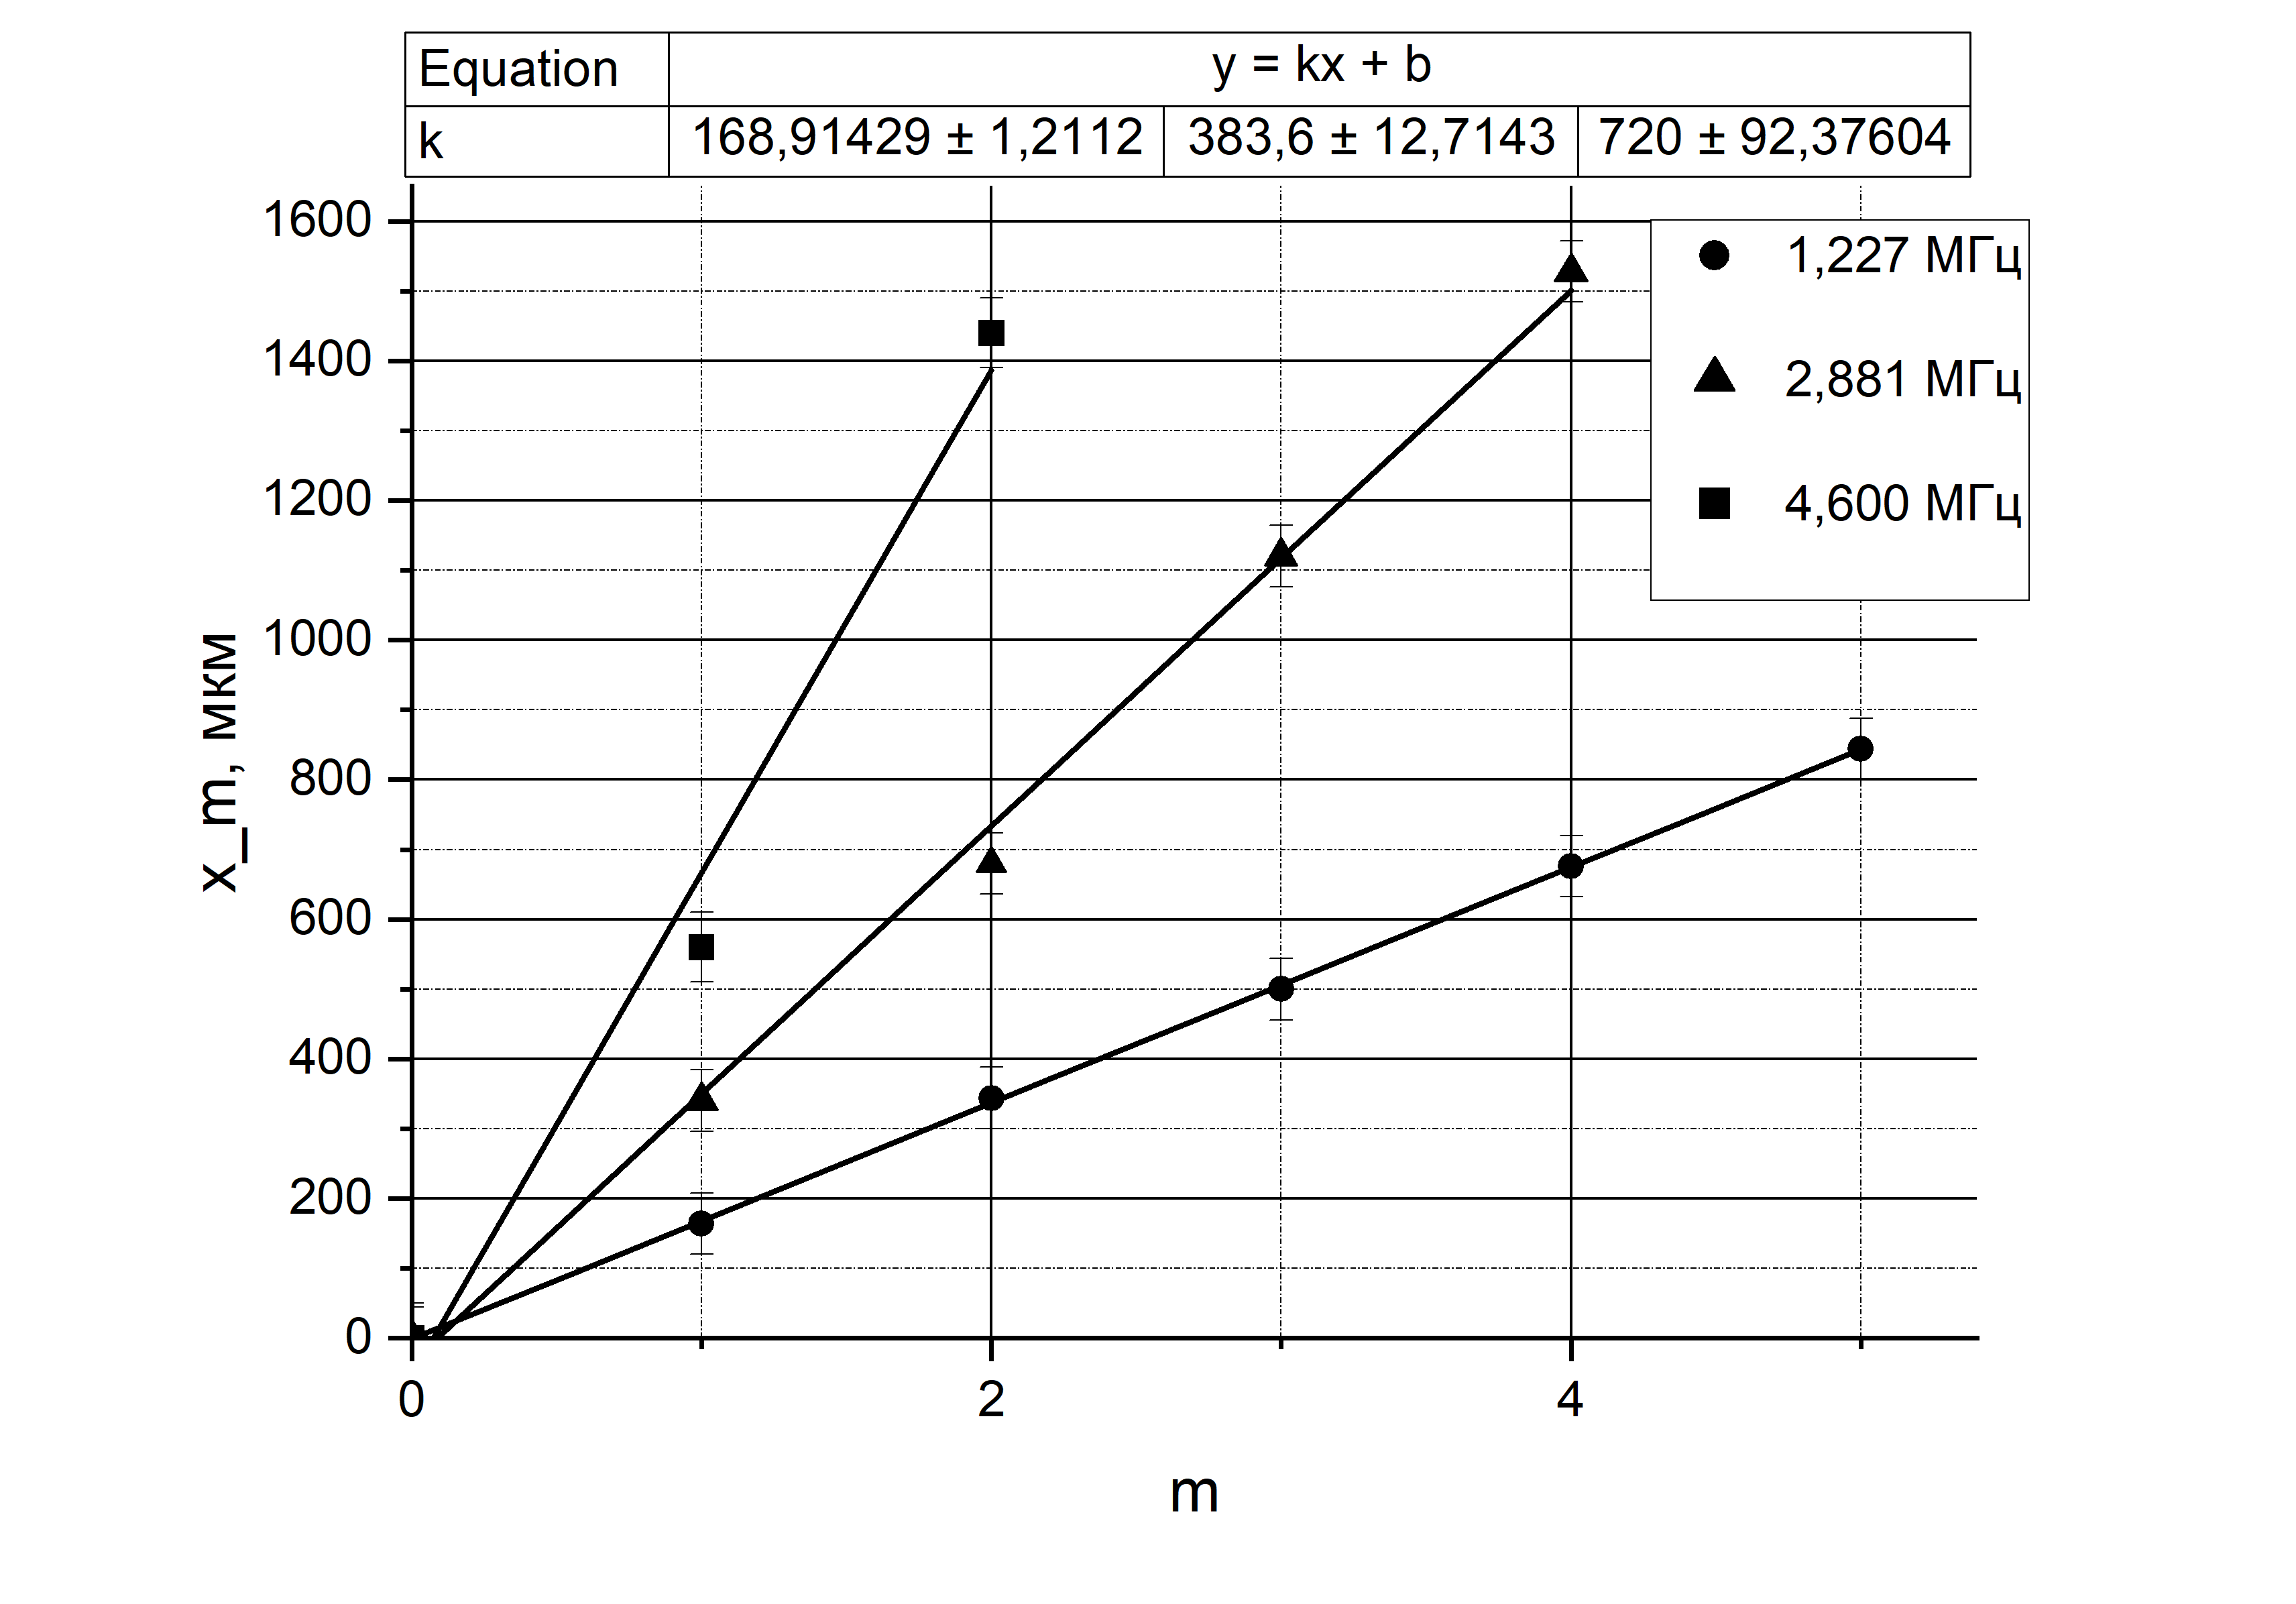
\includegraphics[width=0.8\linewidth]{дифракция.png}
 \end{figure}
 
\noindent 4. Рассчитаем длину $\Lambda$ УЗ-волны по приведенной выше формуле.

\begin{table}[!h]
\begin{tabular}{|l|l|l|l|}
\hline
$\nu, \text{ МГц}$    & 1,227   & 2,881   & 4,6      \\ \hline
$k$                   & 168,9   & 383,6   & 720,0    \\ \hline
$\sigma_k$            & 1,2     & 12,7    & 92,4     \\ \hline
$\Lambda,    \text{ м}$     & 0,00118 & 0,00052 & 0,000276 \\ \hline
$\sigma_\Lambda, \text{ м}$ & 2,1E-05 & 1,9E-05 & 3,57E-05 \\ \hline
\end{tabular}
\end{table}

\noindent 5. Построим график зависимости $\Lambda(1/\nu)$ и определим скорость  ультразвука в воде.

\newpage

\begin{figure}[!h]
 	\centering 	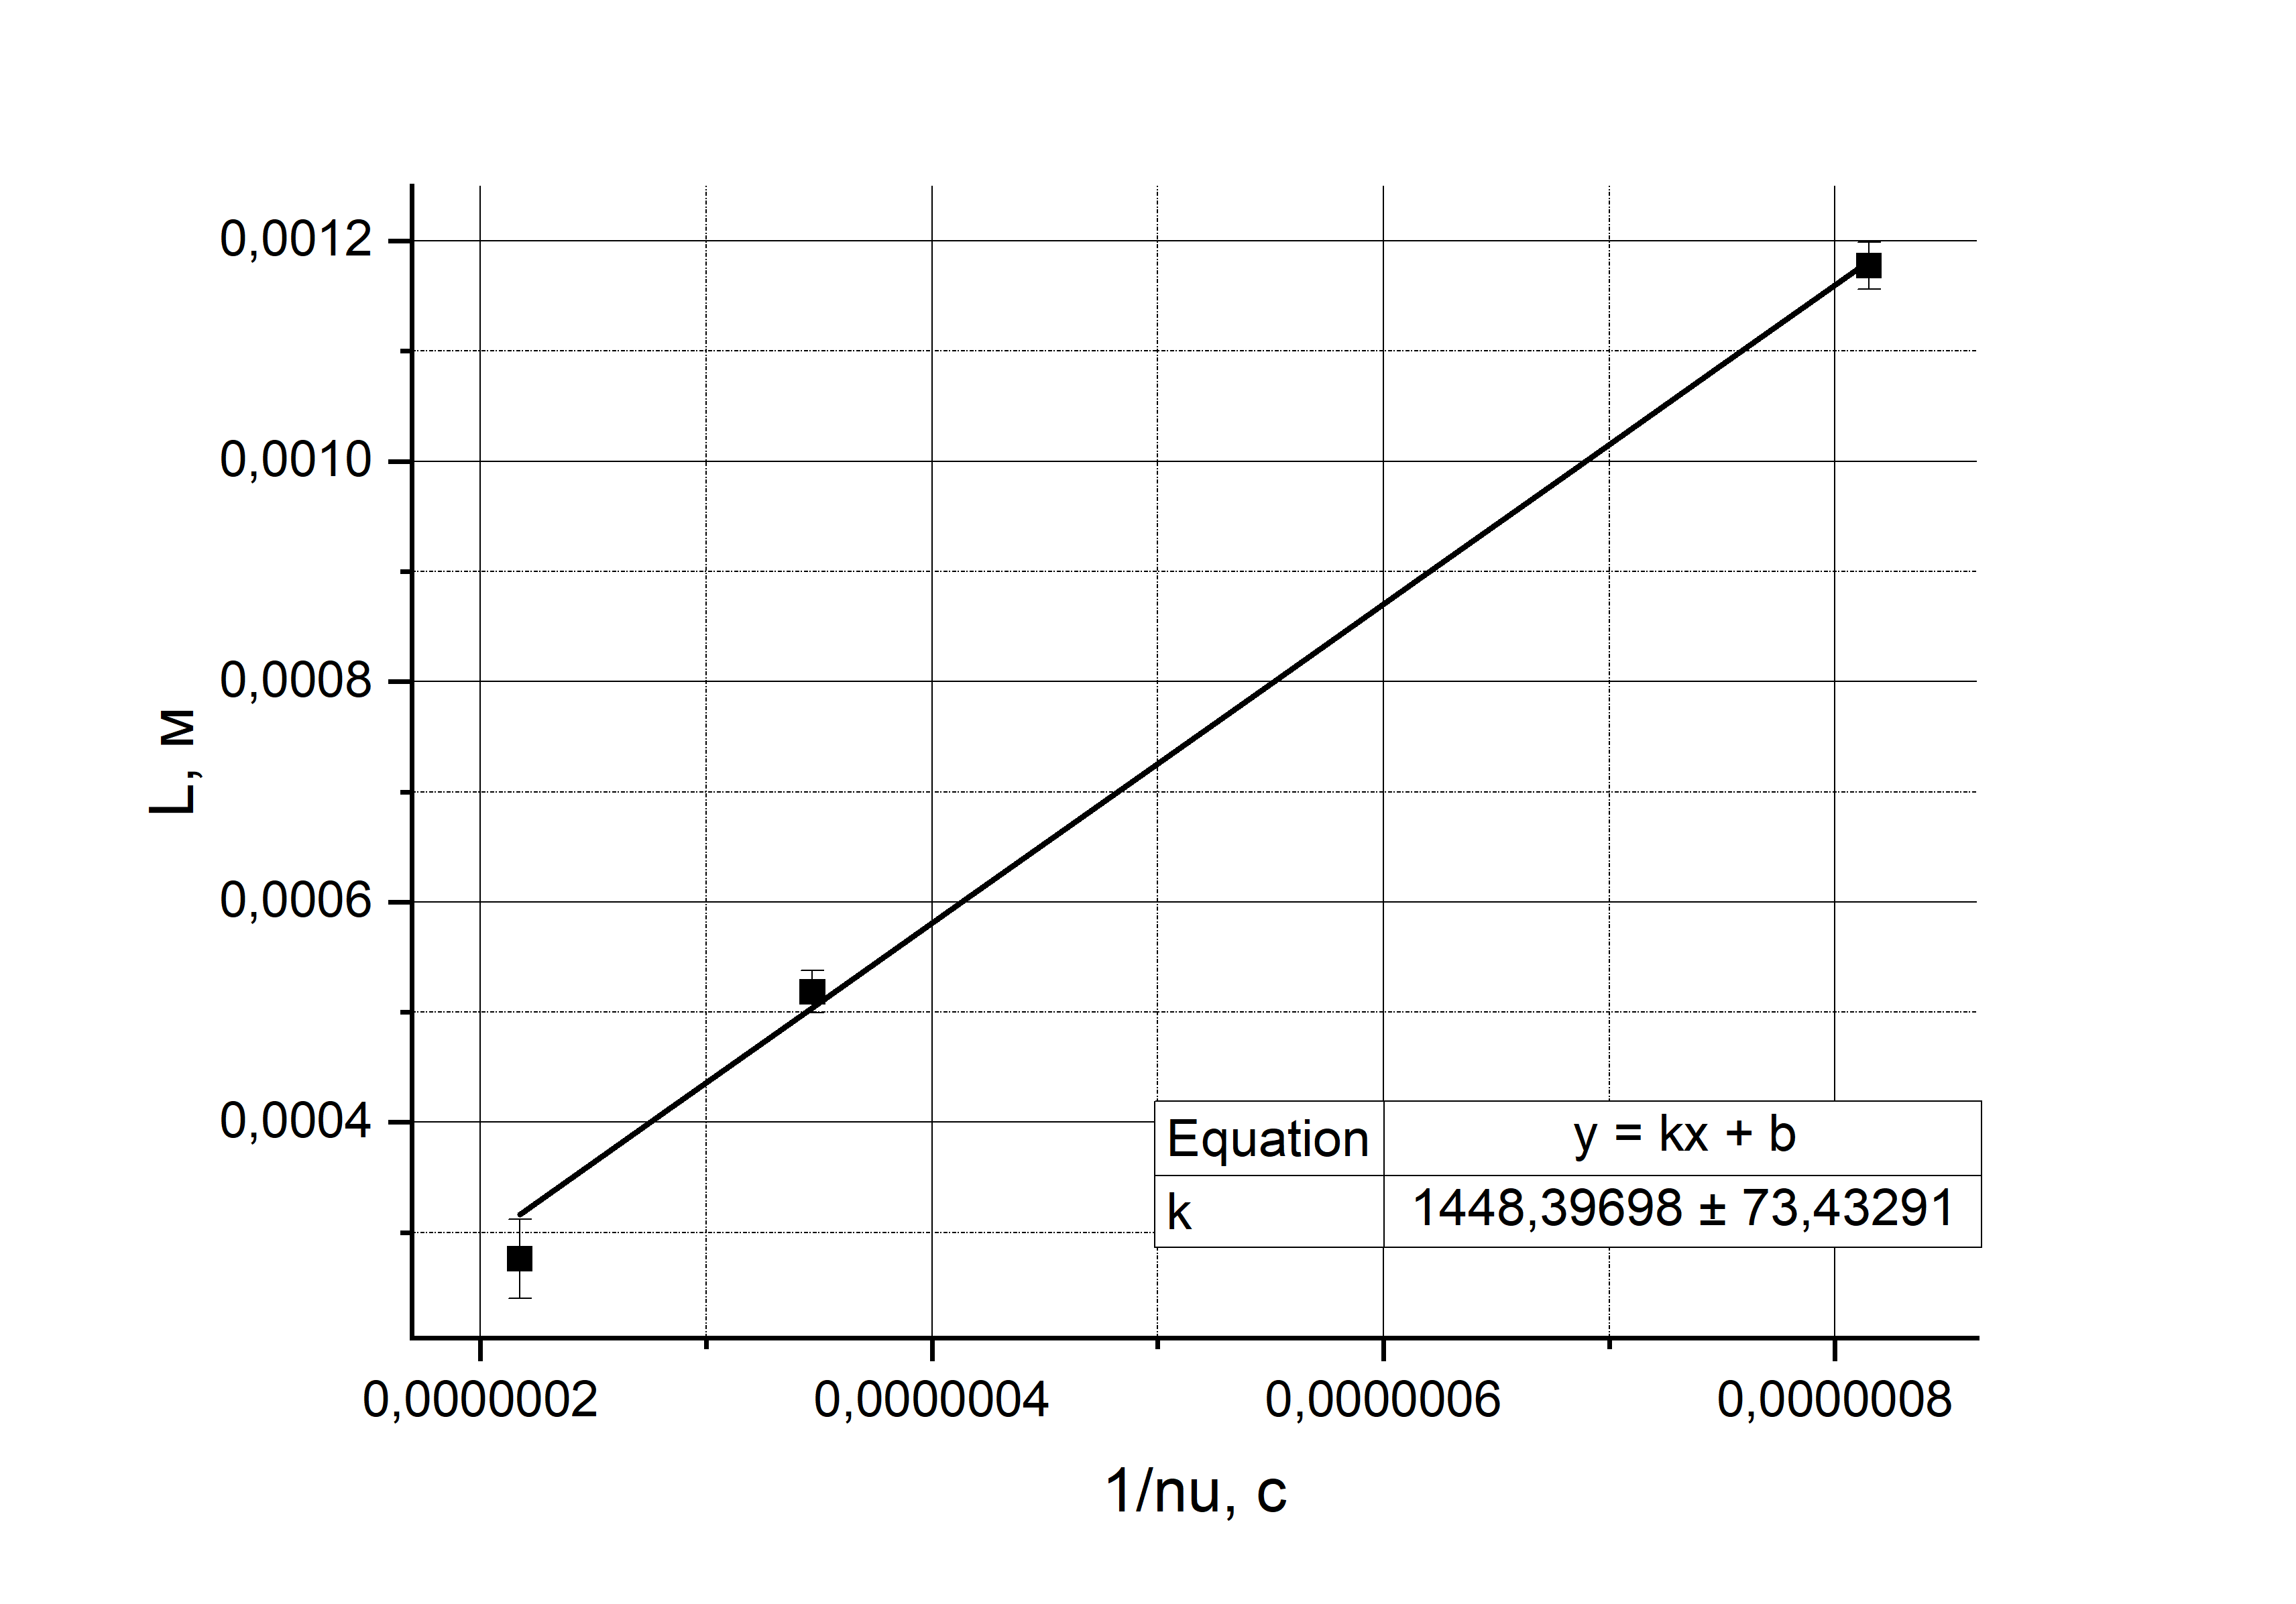
\includegraphics[width=0.8\linewidth]{дифр_2.png}
 \end{figure}
 
\noindent Полученное значение скорости: $v = 1448 \pm 73 \text{ м/с}$.


\subsection{Определение скорости ультразвука методом темного поля}

\begin{figure}[h!]
 	\centering 	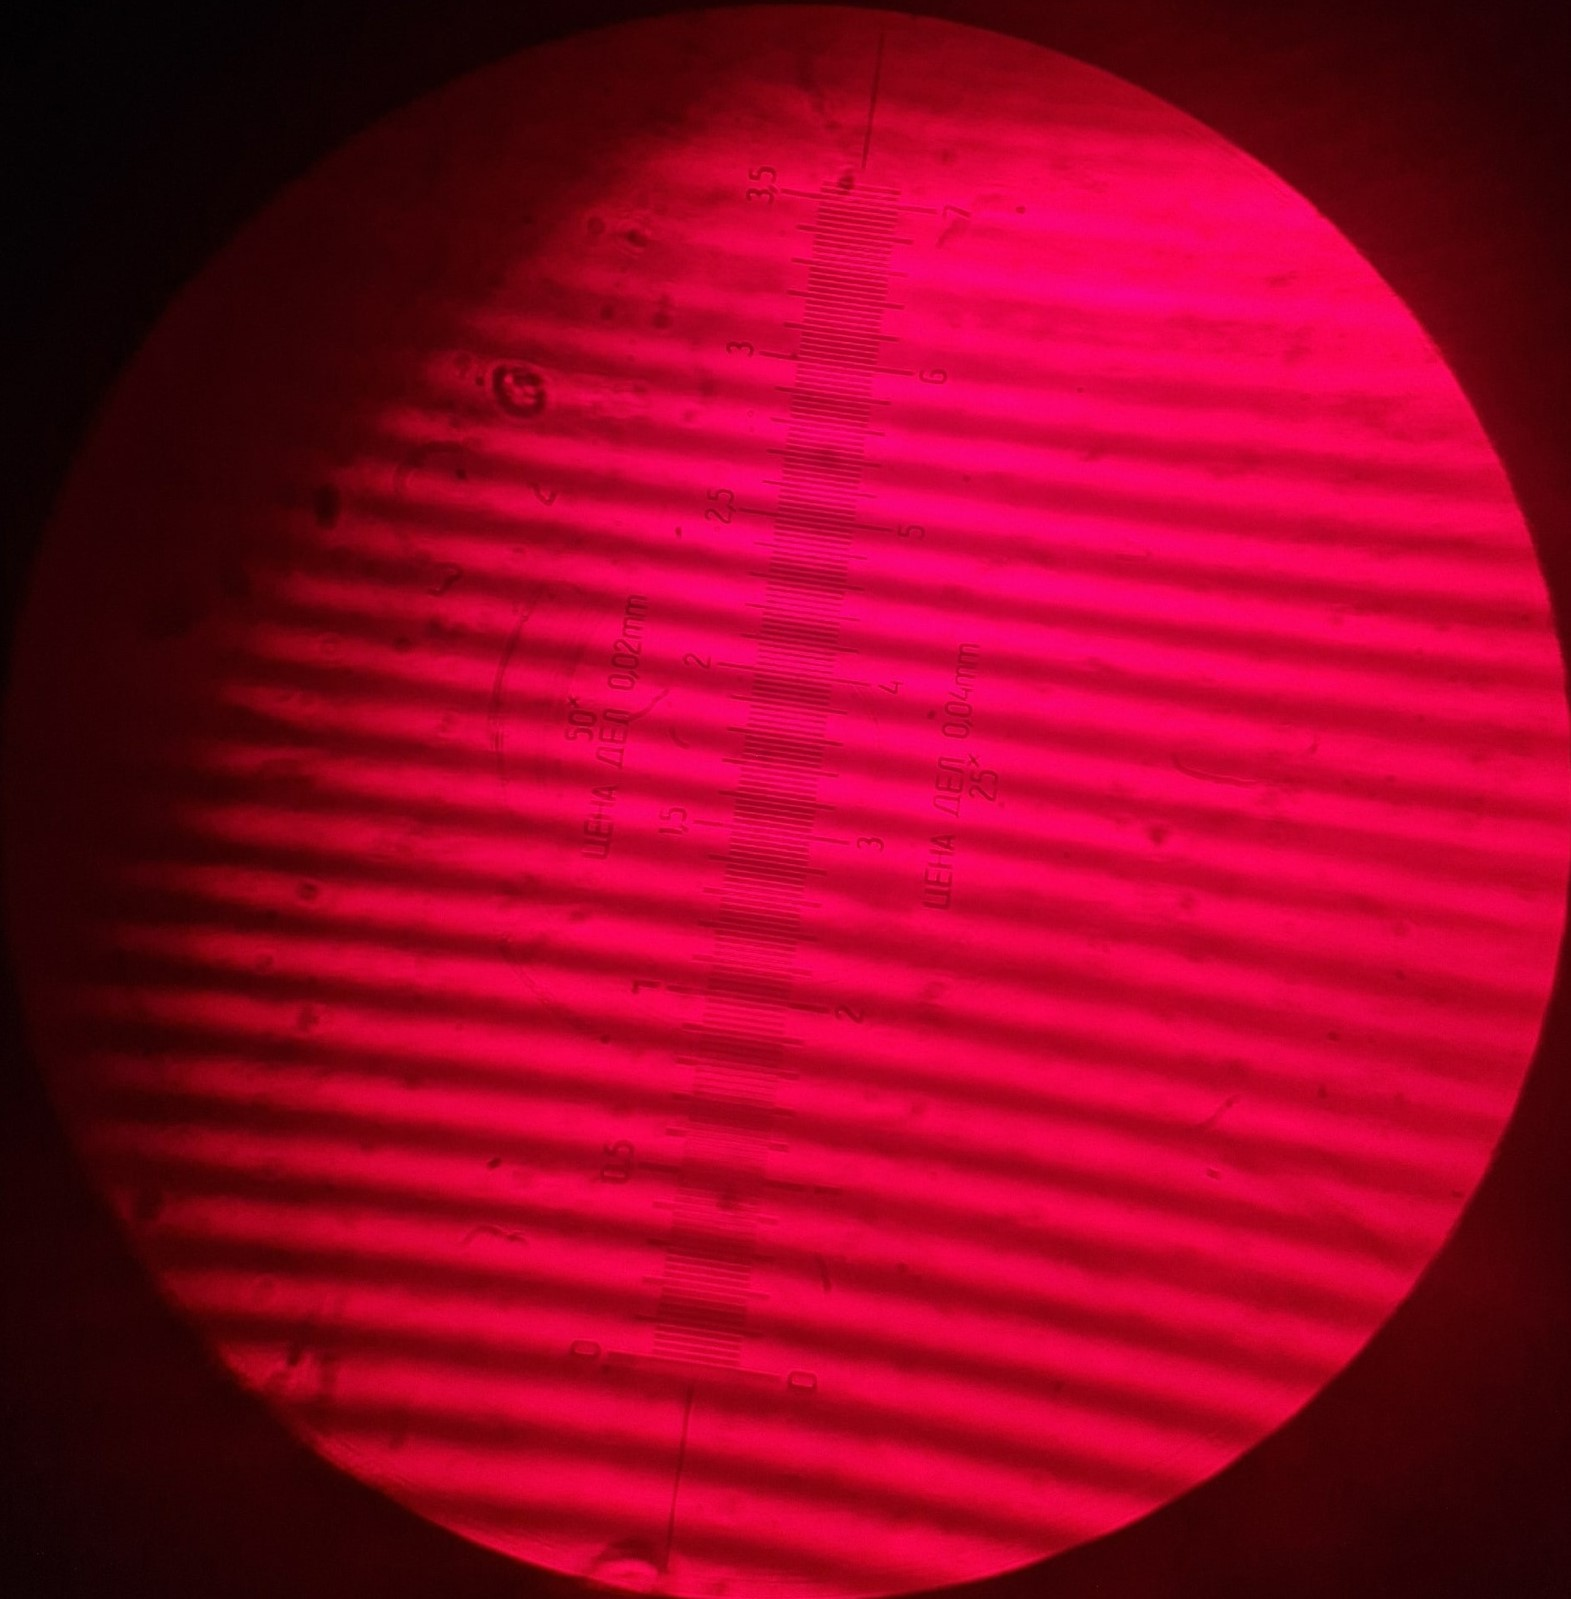
\includegraphics[width=0.4\linewidth]{поле.png}
 \end{figure}

\noindent 1. Введем в поле зрения микроскопа вертикальную нить. Проведем настройку и добьемся полного затемнения поля зрения. 

\medskip

\noindent 2. Включим генератор и найдем изображение акустической решетки. (К сожалению, сделать это на своей установке нам не удалось, поэтому далее будем использовать данные с чужой установки).

\medskip

\noindent 3. С помощью окулярной шкалы измерим расстояние между самыми дальними из хорошо видимых темных полос и просчитаем число промежутков между ними.

\medskip

\noindent Определим длину УЗ-волны в воде.

\begin{table}[!h]
\begin{tabular}{|l|l|l|l|}
\hline
$\nu, \text{МГц}$      & 1,1   & 1,3   & 1,6   \\ \hline
$n, \text{дел}$        & 90    & 93    & 58    \\ \hline
$m, \text{линий}$      & 9     & 12    & 11    \\ \hline
$\Lambda, \text{мкм}$        & 900,0 & 697,5 & 474,5 \\ \hline
$\sigma_\Lambda, \text{мкм}$ & 20,0  & 15,0  & 16,4  \\ \hline
\end{tabular}
\end{table}

\noindent 4. Определим скорость ультразвука по графику $\Lambda(1/\nu)$.

\newpage

\begin{figure}[!h]
 	\centering 	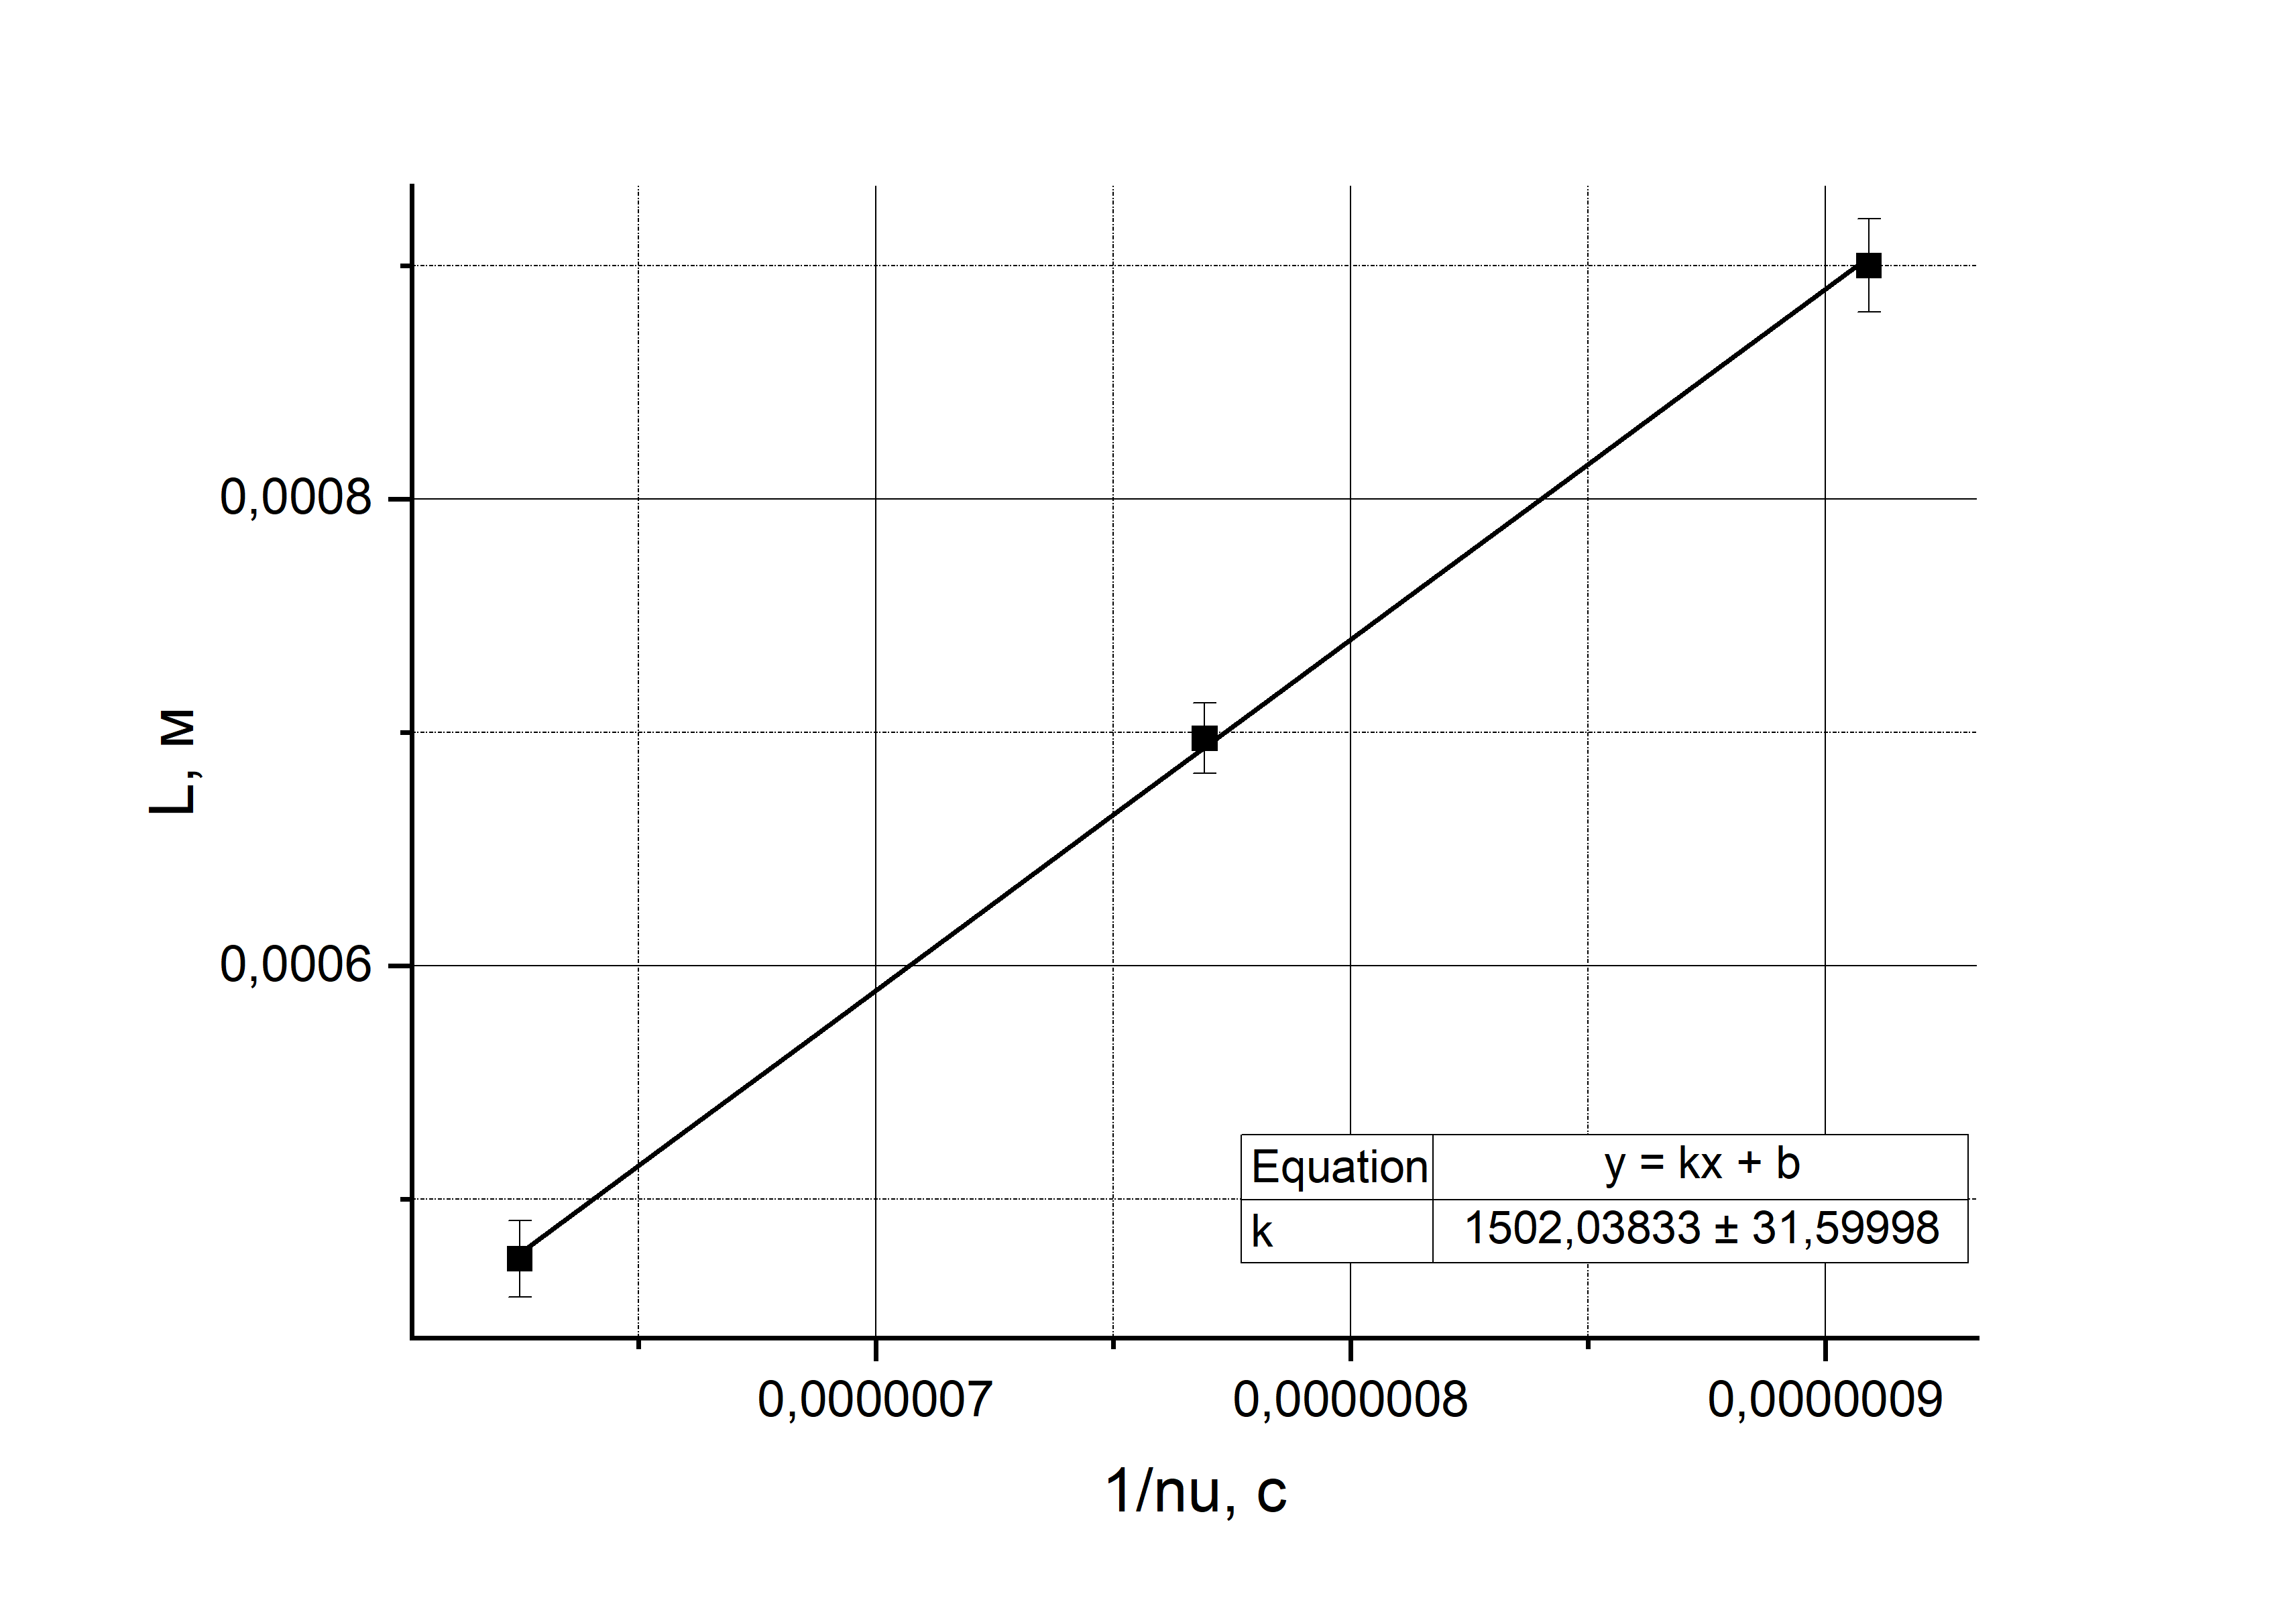
\includegraphics[width=0.8\linewidth]{темное_поле.png}
 \end{figure}
 
\noindent Полученное значение скорости: $v = 1502 \pm 32 \text{ м/с}$.


\section{Вывод}

В ходе работы была изучена дифракция света на синусоидальной акустической решетке. Получено значение скорости ультразвука в воде двумя способами: по дифракционной картине ($1448 \pm 73 \text{ м/с}$) и методом темного поля ($1502 \pm 32 \text{ м/с}$). В обоих случаях значения в пределах погрешности совпадают с табличным: $v_\text{табл} = 1490 \text{ м/с}$ .
 

\end{document}